%!TEX root = ../thesis.tex
%*******************************************************************************
%****************************** Second Chapter *********************************
%*******************************************************************************

\chapter{My second chapter}

\ifpdf
    \graphicspath{{Chapter2/Figs/Raster/}{Chapter2/Figs/PDF/}{Chapter2/Figs/}}
\else
    \graphicspath{{Chapter2/Figs/Vector/}{Chapter2/Figs/}}
\fi

\begin{markdown}

%%%%%%%%%%%%%%%%%%%%%%%%%%%%%%%%%%%%%%%%%%%%%%%%%%%%%%%%%%%%%%%%%%%%%%%%%%%%%%%%%
%%%%%%%%%%%%%%%%%%%%%%%%%%%%%%%%%%%%%%%%%%%%%%%%%%%%%%%%%%%%%%%%%%%%%%%%%%%%%%%%%

## Results

\improvement[inline]{refine subsection title below}
### Benchmarking assembly methods with genomic data from three technologies \label{sec:asm_results}

A central component of the work in this chapter is having a way of validating the quality of variant calls, without being biased by assuming short reads are the "truth". In addition to the matched sequencing on both the \ont{} and Illumina platforms, XXX of the Malagasy samples were also sent for PacBio Circular Consensus Sequencing (CCS)\improvement{clarify this from the methods Sara sent - i.e. is HiFi more correct?}. CCS produces so called HiFi reads, which have a base-level accuracy greater than 99.9\%(CITE). The reason these reads have such a high accuracy is that each one is the consensus from multiple passes of the DNA enzyme around a circular copy of the original double-stranded read. As the HiFi reads are both long and accurate, they are now being regularly used to produce high quality \denovo{} assemblies and complete existing reference genomes(CITE).  

Due to the lack of extensive benchmarking of assembly methods for CCS, and \mtb{} more generally, we undertook to determine what combination of technologies and methods would give us the best "truth" genomes. There has been comprehensive analysis of \ont{} and hybrid assemblies for \ecoli{}(CITE), but its genomic characteristics are very different to those of \mtb{}. For this analysis we chose to assess five assemblers: `flye`, `canu`, `spades`, `unicycler`, and `HASLR`(CITE). Both `unicycler` and `HASLR` are hybrid assemblers, which means they utilise both long and short reads. We use them to produce Illumina/CCS and Illumina/\ont{} assemblies. The only tool capable of operating with all three technologies (at the time of writing) is `spades`. One assembly for each long read technology was produced with `canu` and `flye`.  
Each assembly was additionally polished with their relevant long reads and Illumina data using `racon` and `pilon` respectively. These combinations resulted in 18 assemblies (9 polished and 9 unpolished) for assessment.  

Assessing the quality of \denovo{} assemblies is non-trivial and requires aggregation of various metrics(CITE). Whilst a reference genome exists for \mtb{}, there are enough differences between the lineages that using this reference would not be appropriate for our purposes. We will look at each assessment metric individually, and then decide on the best assembly method from this information

#### Assembly Likelihood Evaluation score

The assembly likelihood evaluation (ALE) score is a reference-free metric that describes the likelihood of an assembly given it's k-mer distribution, and the likelihood of the reads being generated from that assembly. It combines information such as read quality, agreement in the alignment of reads to assembly, mate-pair orientation, paired-end read length, and depth of sequencing. Importantly, the ALE score can be used to compare assemblies of the same genome, which is exactly the use case we have. Whilst ALE scores and not insightful on their own, the difference \textit{between} assembly scores gives the relative probability of correctness. So for each sample, we are interesting in the assembly that has the \textit{highest} ALE score.  

Across the 9 samples, `flye` has the highest ALE score in five cases, whilst `spades` was the most probable assembly in two, with `unicycler` and `canu` having the maximum score in one sample each (\autoref{fig:ale_score}). Note, this is considering both polished and unpolished assemblies together for each tool. When considering which long read sequencing technology produces the greatest ALE score, CCS had the top score in 7/9 samples. In 6/9 samples, the highest ALE score was from a polished assembly.\unsure{is this figure necessary or are the numbers in the text sufficient?}

\end{markdown}

\begin{figure}
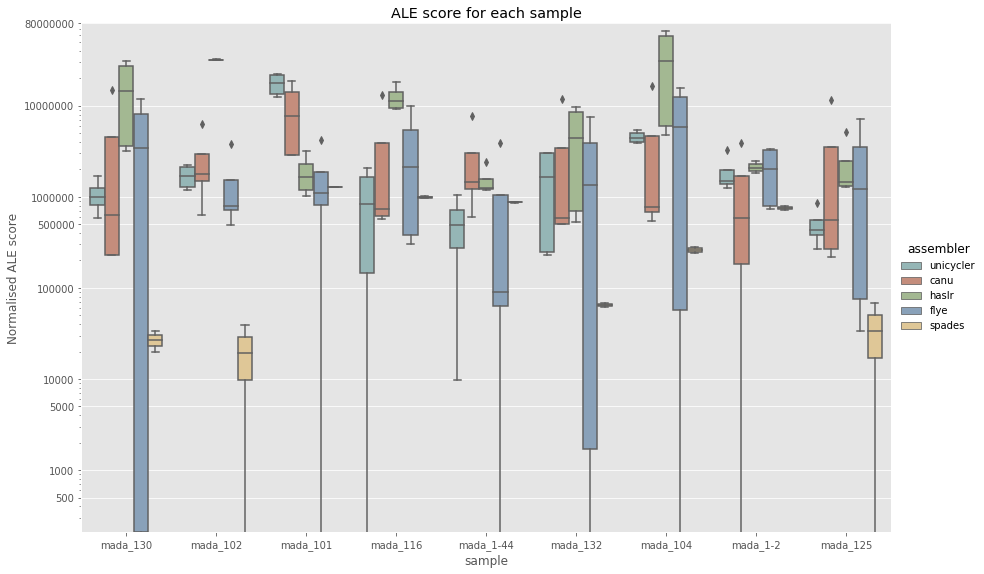
\includegraphics[width=1.0\textwidth]{Chapter2/Figs/ale_score.png}
\centering
\caption{The normalised ALE score (Y-axis) for each sample (X-axis), coloured by assembly tools. ALE score is a metric describing the likelihood of an assembly. The normalisation is done by subtracting the assembly's score from the maximum (best) score for that sample, giving a relative probability of correctness. Each box represents different technologies and polishing status for each assembler.}
\label{fig:ale_score}
\end{figure}

\begin{markdown}

#### Disagreement rate

The disagreement rate is an approximation of the per-base accuracy of the assembly (see Methods\todo{link to relevant methods section}). In short, we map Illumina reads to the assembly and calculate what proportion of positions do XXX\% of the reads agree with the assembly nucleotide.  

In 7/9 samples, a `HASLR` assembly had the lowest disagreement rate, followed by `unicycler` having the minimum in 2/9. Polished genomes produced the lowest disagreement rate in 8/9 samples and \ont{}-based assemblies had the best accuracy in 6/9 samples. While it isn't so surprising that assemblies polished with Illumina reads have a lower disagreement rate, it is unexpected that \ont{} would produce more accurate assemblies (\autoref{fig:disagree_rate}). One caveat to keep in mind here - and this is the reason for looking at many different metrics - is that there is an element of overfitting to this metric: we assess using Illumina, and so naturally, assemblies polished with Illumina produce better results. That is not to say this statistic is void, but that it should be used with caution.

\end{markdown}

\begin{figure}
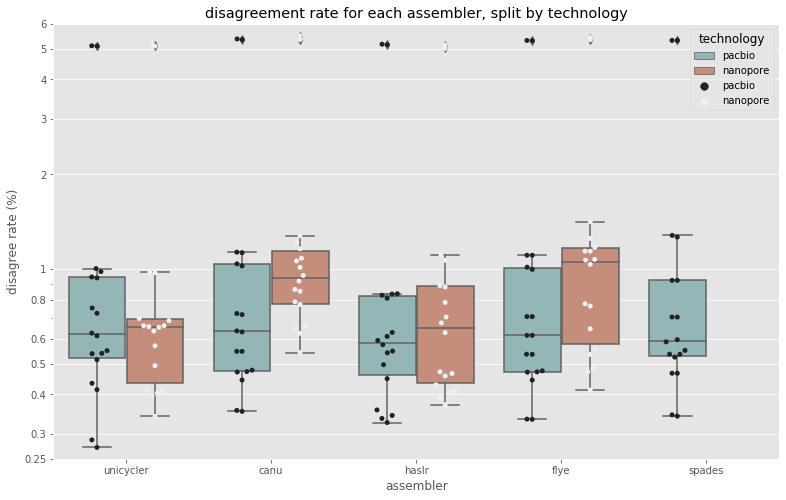
\includegraphics[width=1.0\textwidth]{Chapter2/Figs/disagree_rate.png}
\centering
\caption{The disagreement rate (Y-axis) for each assembler (X-axis), coloured by the sequencing technology. Disagreement rate is the percentage of sites in the assembly where Illumina reads do not have XX\% quorum. Each box/point represents different samples and polished status for the relevant assembler-technology combination.}
\label{fig:disagree_rate}
\end{figure}

\begin{markdown}

#### Number of contigs

As \mtb{} has only a single, circular chromosome, for an assembly to be structurally complete, there should only be a single contig in the final assembly. However, it is not always appropriate for an assembly method to produce a single contig as data quality, depth of sequencing, read length, and/or repetitive content of the genome can hamper this goal(CITE). Conversely, receiving a single contig as output is no guarantee of it's quality for similar reasons to the previous, multi-contig scenario. For the purposes of this benchmark, considering on conjunction with the other metrics, the number of contigs can be a useful datum for selecting our favoured assembly. If an assembly has a single contig, and scores well on other metrics, we would be more inclined to choose it over another assembly with similar metrics, but many more contigs.

Across all combinations of assembly conditions, `spades` (8/18), `flye` (18/32) and `canu` (16/32) produced far more single-contig assemblies than the hybrid methods (\autoref{fig:num_contigs}). `unicycler` produced no single-contig genomes, whilst `HASLR` yielded only 2/32. When considering sequencing technology, CCS (26/72) had many more single-contig assemblies than \ont{} (10/72). Note: `spades` assemblies use all three technologies and are not considered in the technology single-contig totals.

\end{markdown}

\begin{figure}
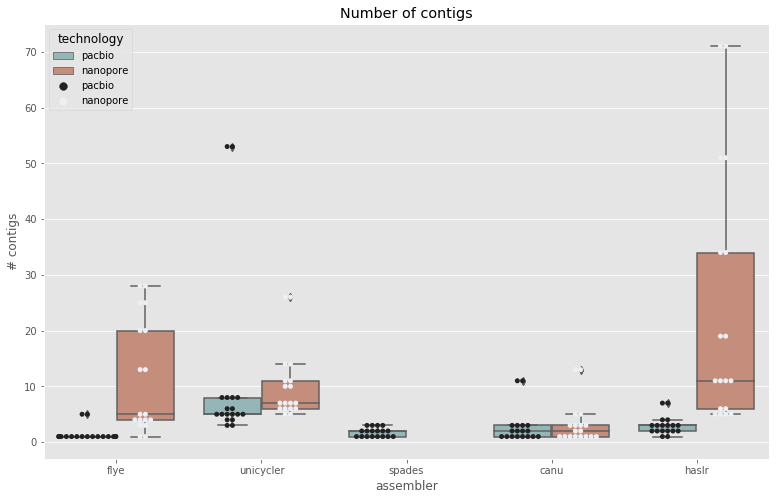
\includegraphics[width=1.0\textwidth]{Chapter2/Figs/num_contigs.png}
\centering
\caption{The number of contigs (Y-axis) produced from each assembly (X-axis), coloured by sequencing technology. Each box/point represents different samples and polished status for the relevant assembler-technology combination.}
\label{fig:num_contigs}
\end{figure}

\begin{markdown}

#### Length of assembly

As mentioned earlier, comparing the assemblies to the \mtb{} reference genome (H37Rv; accession: `NC_000962.3`) is not appropriate, however, it's length/size can be used as an aid for selection. The size of the any lineage's genome is not expected to differ from the reference by more than about X kilobases(CITE). Considering the genome size in addition to disagreement rate is particularly informative. It would be quite easy for an assembly method to produce very accurate per-base contigs but refusing to produce sequence for "harder" parts of the genome. While such an assembly would score well on disagreement rate, it would not do so well when considering how close to the expected genome size it is. The length of the assembly is also clearly shows when a method is outputting \textit{too much} sequence.

When comparing the size of each assembly to that of H37Rv, we found a fairly even spread across assemblers for the closest size to H37Rv. For 3/9 samples, `canu` has the smallest size difference, followed by `spades` (2/9), `unicycler` (2/9), `HASLR` (1/9) and `flye` (1/9). An honourable mention should be made of `flye` and `spades` as they had much lower variation in size compared to the other approaches. In terms of sequencing technology, in 6/9 samples CCS produced the genome size closest to H37Rv. Polished assemblies had the closer size in 5/9 samples.

\end{markdown}

\unsure[inline]{should I use the non-zoomed version of \autoref{fig:asm_len}?}
\begin{figure}
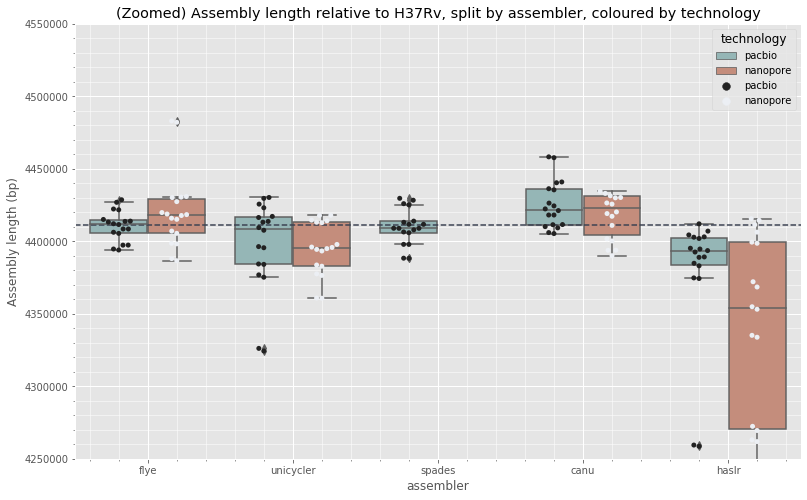
\includegraphics[width=1.0\textwidth]{Chapter2/Figs/asm_len.png}
\centering
\caption{Size/length (Y-axis) of each assembly (X-axis), coloured by each sequencing technology. The horizontal dashed line represents the size of the \mtb{} reference genome (4,411,532bp). Each box/point represents different samples and polished status for the relevant assembler-technology combination. Note: the Y-axis has been limited to allow for greater resolution of similarity to the H37Rv size}
\label{fig:asm_len}
\end{figure}

\begin{markdown}

#### Contamination detection

The decontamination step in the assembly pipeline (\todo{reference relevant section in methods}) revealed that one sample, `mada_1-2`, contained contigs from three different species: *Mycobacterium intracellulare*, *Dermacoccus nishinomiyaensis*, and *M. tuberculosis*. These contigs were all at sufficient coverage to not be considered background noise. For the assembly assessment analysis only the contigs from \mtb{} were used, but figures for the assessment metrics in the previous subsections show this sample is an outlier in almost all metrics. Given this profuse contamination, `mada_1-2` will not be used in any analysis where these assemblies are used for truth validation purposes.

\\

\unsure{should this paragraph stay here or move to the conclusion?}In conclusion, considering all assessment metrics, `flye` and `spades` assemblies were consistently the better performing methods across all of the criteria outlined in this section. As most of the validation analyses that these assemblies will be used for involve comparing Illumina and \ont{} data to a "neutral truth", the unpolished CCS assemblies from `flye` were selected for use in the remainder of this chapter. The differences between the polished and unpolished CCS assemblies was almost negligible and do not outweigh the benefit of having a single-technology PacBio assembly that can be used as an unbiased reference point for comparing the other two technologies.

%%%%%%%%%%%%%%%%%%%%%%%%%%%%%%%%%%%%%%%%%%%%%%%%%%%%%%%%%%%%%%%%%%%%%%%%%%%%%%%%%

### An \mtb{} species-specific \ont{} basecalling model improves accuracy

It has previously been shown(CITE) that a taxon-specific basecalling model can improve both the read-level and consensus accuracy of \ont{} sequencing reads. While this was shown for *Klebsiella pneumoniae*, it remains to be seen if this approach generalises to other species. The major difficulty in producing such a model pertains to the requirement for a "truth" genome for the training data. The \ont{} basecaller, \guppy{}, uses neural networks to convert raw signal into a DNA sequence. In order to train the network in how to make this inference it is necessary to label the raw signal with its corresponding "truth" sequence. Such datasets are difficult to find for certain species. However, the dataset we have collected for the work in this chapter is perfectly suited as we have reads from Illumina, PacBio, and \ont{} that are from the *exact* sample DNA extraction. As the bulk of the work in this chapter (and the subsequent chapters) has an implicit reliance on the quality of the \ont{} basecalling accuracy, we sought to train a \mtb{}-specific \guppy{} model.  

To facilitate the training of the \mtb{}-specific model we used the \ont{} model-training tool \taiyaki{} (see \todo{add link to relevant methods section}). We use the samples with matched PacBio data for the training as they have high quality assemblies that can be used as truth (\autoref{sec:asm_results}). With the aid of \taiyaki{} we map the basecalled \ont{} reads to the truth assembly; creating a truth sequence for each read. The truth sequence for each read is then mapped to the raw signal, which is the main input format for training. Across the eight samples there was a total of 1,309,049 \ont{} reads that were mapped. Reads were split into training (20\% - 261,808 reads) and evaluation (80\% - 1,047,241 reads) sets. The model was trained by \taiyaki{} (using only the training set) and took 108 hours (4.5 days) to complete on 2 GPUs. The resulting \mtb{} model (referred to as 'tubby') was then used to re-basecall the reads in the evaluation set. We evaluate the tubby model and the default \guppy{} model inline with Wick *et al.*(CITE)(see \todo{add link to relevant methods section}).

#### Read BLAST identity

The first evaluation metric, read BLAST identity, determines the read-level accuracy produced by the basecalling model. We align the basecalled reads to the truth assembly and calculate BLAST identity as, for each mapping, the number of matching bases divided by the length of the alignment. \autoref{fig:combined_basecall}A shows the tubby model has a higher read-level BLAST identity (median 0.941) than \guppy{} (median 0.920).

#### Relative read length

We define relative read length as the length of the aligned part of the read, divided by the total length of the read. The purpose of this metric is to see whether there is a bias towards insertions (greater than 1.0) or deletions (less than 1.0). \autoref{fig:combined_basecall}C shows that, at the read level, tubby has a slight tendency towards deletions (shorter reads) compared to \guppy{} with median relative read lengths of 0.982 and 0.993 respectively. However, this result is a little more complex than just looking at median values. The distribution of lengths for \guppy{} extends much further past 1.0 compared with tubby, indicating an increase in insertions. We will return to this result when we look at the error types.

#### Consensus accuracy

To assess consensus accuracy the basecalled reads were assembled using `rebaler`. `rebaler` was developed by Wick *et al.* for the purposes of evaluating basecalling models and is a reference-guided assembly approach (see \todo{link to relevant methods section}). Here we show consensus accuracy in a similar manner to read identity. Each "read" in this context is the result of chopping the `rebaler` assembly of the reads up into 10kbp "chunks" to simulate reads. These chunks are then mapped back to the original assembly and we use BLAST identity as the measure of accuracy. \autoref{fig:combined_basecall}B shows tubby has higher consensus accuracy (median 0.9993) compared with \guppy{} (median 0.9992). The consensus accuracy improvement of 0.0001 equates to approximately 440 less erroneous positions in the \mtb{} assembly.

\end{markdown}

\begin{figure}
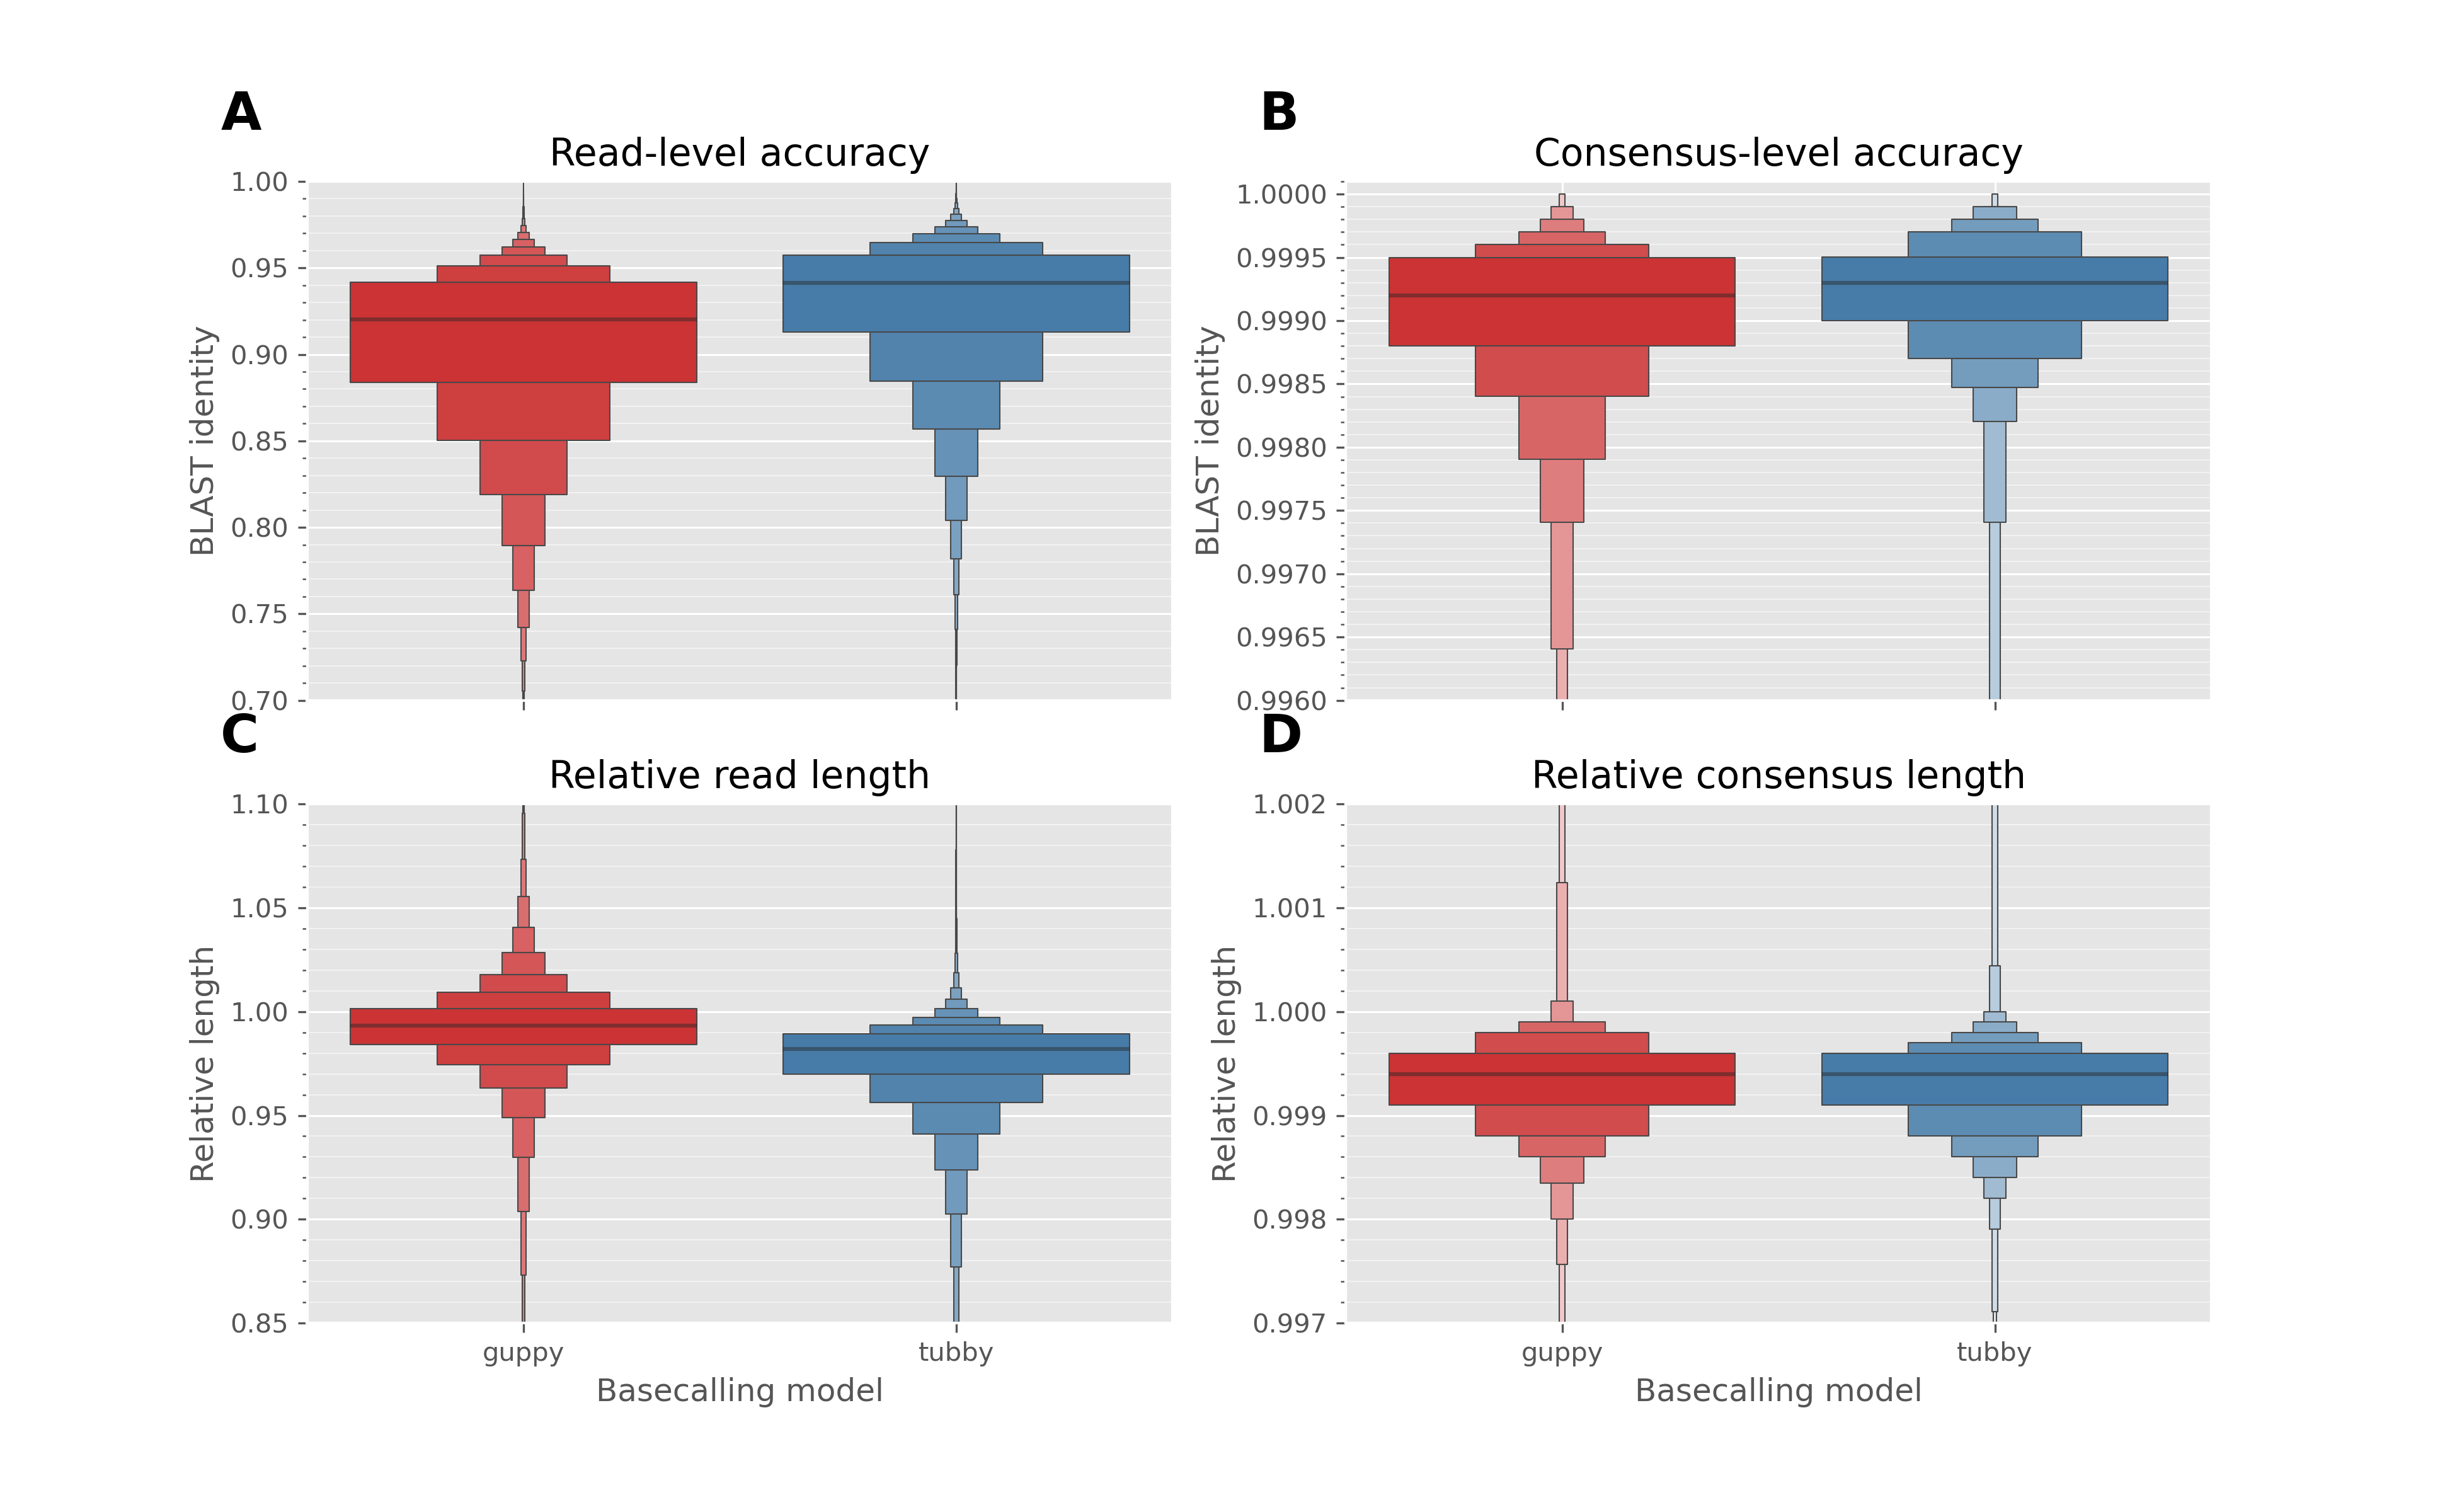
\includegraphics[width=1.0\textwidth]{Chapter2/Figs/combined_identity_relative_len.png}
\centering
\caption{A) Read BLAST identity (Y-axis) for the \mtb{}-specific basecalling model 'tubby' (blue) compared with the default \guppy{} model (red). BLAST identity is the number of matching bases (in a read alignment) divided by the length of the alignment. B) Consensus BLAST identity (Y-axis), where consensus refers to "chunks" of the genome assembly produced by the basecalled reads, for each model, mapped to the truth genome. C) Relative read length (Y-axis) for the two models. Relative read length is the length of the aligned part of the read, divided by the total length of the read. D) Consensus relative length. Relative length is the length of the aligned part of the consensus "chunk", divided by the total length of the "chunk". Note: the Y-axes have all been zoomed-in to allow closer inspection of the majority of data.}
\label{fig:combined_basecall}
\end{figure}

\begin{markdown}

#### Error types

Here we classify the types of errors that occur in the `rebaler` assemblies and look at how these errors compare across models. To determine the errors, we categorise the differences between the truth and `rebaler` assemblies (see \todo{link to relevant methods}). \autoref{fig:error_types} shows that the greater part of the error types (for both models) are attributable to deletions, with most being homopolymer deletions. We do however see that, except for non-homopolymer deletions, tubby's errors are lower than \guppy{}'s \todo{add some concrete numbers}. In the case of both insertion types, tubby has approximately 3.5-fold less insertions than \guppy{} - although these constitute a small portion of the overall errors. Both models have a very low level of Dcm-methylation errors, which is a nice control of sorts as \mtb{} does not have any known 5-methylcystosine methyltransferases(CITE)\improvement{ensure the wording of this and correct and that the claim is also correct}.

\end{markdown}

\begin{figure}
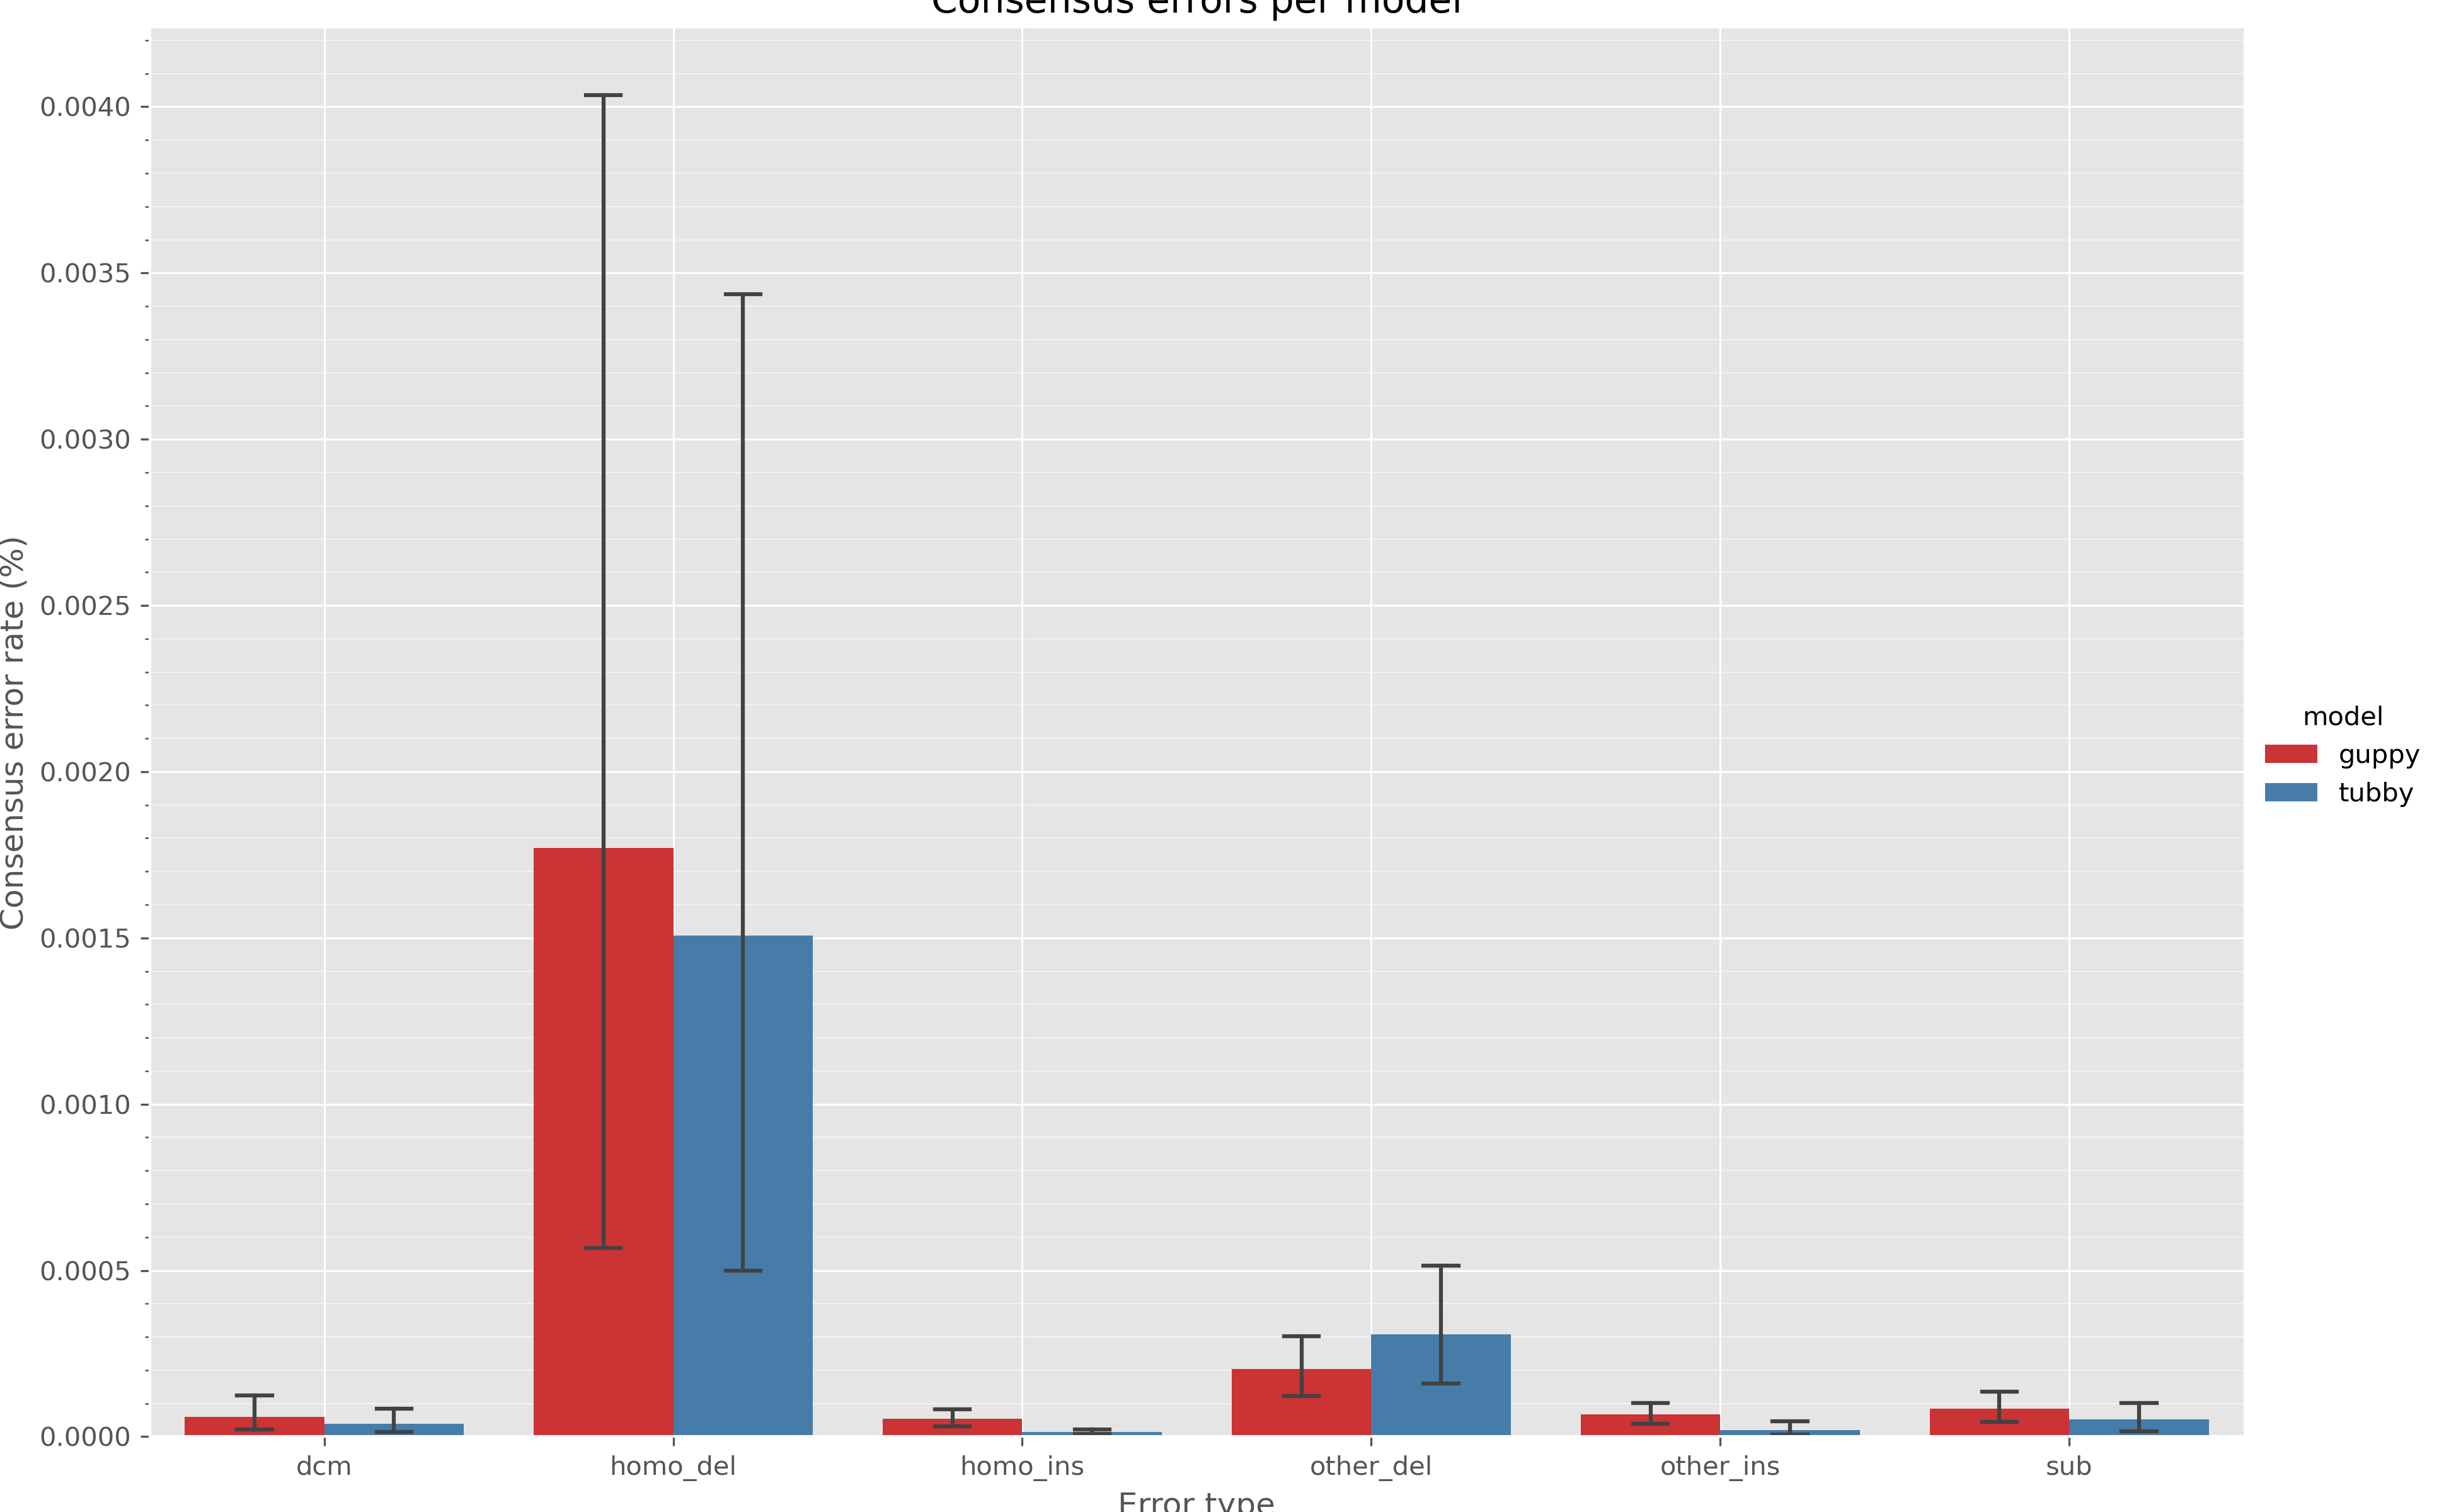
\includegraphics[width=1.0\textwidth]{Chapter2/Figs/consensus-error-types.png}
\centering
\caption{Error types in the `rebaler` assemblies produced from reads basecalled with tubby (blue) and \guppy{} (red). The consensus error rate is the percentage of the assembly these errors compose. The errors are per-assembly, so the confidence intervals represent variation in error types between samples/assemblies. dcm refers to Dcm-methylation motifs. homo\_ins/del are homopolymer insertions or deletions. sub is single-base substitutions.}
\label{fig:error_types}
\end{figure}

\begin{markdown}

\\

Given the improved performance across nearly all metrics for a \mtb{}-specific \ont{} basecalling model, tubby will be used for the remainder of this work. 

%%%%%%%%%%%%%%%%%%%%%%%%%%%%%%%%%%%%%%%%%%%%%%%%%%%%%%%%%%%%%%%%%%%%%%%%%%%%%%%%%

### Quality Control

The purpose of QC is to ensure all samples used in later analysis are of the highest quality. By highest quality we mean all samples have perfectly matched Illumina and \ont{} data, sufficient coverage on both sequencing technologies, no contamination, and no evidence of a mixed \mtb{} population. Prior to the QC stage, N samples were excluded as their Illumina and \ont{} reads were not from the exact same DNA extraction.  

After filtering out unmapped/contaminant reads and subsampling all samples to 60x (Illumina) and 150x (\ont{}), N samples were excluded from further analysis due to low coverage (FIGURE) - defined as Nx for Illumina and Nx for \ont{}. An example chart of the composition of genomes from the decontamination database for a sample can be seen in (FIGURE).  

Lastly, N samples were excluded as their lineage assignment was either called mixed or unknown. Unknown lineage assignments can happen if the sample has too many heterozygous calls as lineage-defining positions, or there was no called lineages at any lineage-defining position.  

In the end, we have N samples that have passed QC and will be used for the remainder of this chapter.

\missingfigure{coverage report from QC pipeline - maybe add coverage cutoff lines}
\missingfigure{An example Krona composition chart}

\towrite[inline]{Make sure to mention the samples excluded as their Illumina and ONT data do not match based on the discrepancy in variant calls}

%%%%%%%%%%%%%%%%%%%%%%%%%%%%%%%%%%%%%%%%%%%%%%%%%%%%%%%%%%%%%%%%%%%%%%%%%%%%%%%%%

\improvement[inline]{refine subsection title below}
### Building PRGs of varying density

%%%%%%%%%%%%%%%%%%%%%%%%%%%%%%%%%%%%%%%%%%%%%%%%%%%%%%%%%%%%%%%%%%%%%%%%%%%%%%%%%

### \ont{} SNPs are highly concordant with Illumina

%%%%%%%%%%%%%%%%%%%%%%%%%%%%%%%%%%%%%%%%%%%%%%%%%%%%%%%%%%%%%%%%%%%%%%%%%%%%%%%%%

### Genome graphs provide superior \ont{} indel calls compared to a pileup approach

%%%%%%%%%%%%%%%%%%%%%%%%%%%%%%%%%%%%%%%%%%%%%%%%%%%%%%%%%%%%%%%%%%%%%%%%%%%%%%%%%

### \ont{} data identifies transmission clusters inline with Illumina

%%%%%%%%%%%%%%%%%%%%%%%%%%%%%%%%%%%%%%%%%%%%%%%%%%%%%%%%%%%%%%%%%%%%%%%%%%%%%%%%%
%%%%%%%%%%%%%%%%%%%%%%%%%%%%%%%%%%%%%%%%%%%%%%%%%%%%%%%%%%%%%%%%%%%%%%%%%%%%%%%%%

## Methods

### Nanopore data preprocessing

All \ont{} data for this project was basecalled and de-multiplexed using the \ont{} proprietary software tool \guppy{} (v3.4.5). We used default parameters for basecalling and the only non-default parameter used for de-multiplexing was the 'trim barcodes' option.  
Quality metrics for assessing whether each sample should be included in the study included read length distribution and coverage (FIGURE). To calculate coverage, we sum the number of base pairs for a sample and divide this by the \mtb{} genome size of 4,411,532bp.

\missingfigure{A plot showing the quality metrics for \ont{} data such as read length distribution and coverage}

### Assembly

Samples with greater than 30x coverage across all three sequencing technologies were chosen to produce high-quality assemblies. In total, this left us with 9 Malagasy samples. We compare five assemblers and select the best for each sample. The reason for this comparison is that different assembly algorithms can produce quite varied results depending on sequencing technology used, species, or computational resource availability(CITE).  
The assembly tools used are Canu, Flye, Unicycler, HASLR, and Spades(CITE \& VERSION). HASLR and Unicycler are hybrid assemblers that take Illumina reads along with one long-read file, although Unicycler does not require both. Spades is also a hybrid assembler but takes an arbitrary number of different sequencing technologies. Canu and Flye are both long-read-only assemblers.

The entire assembly pipeline was orchestrated using the workflow management system Snakemake(CITE). An overview of the entire pipeline is shown in (FIGURE). The first step is trimming of adapter sequences in the Illumina reads using Trimmomatic(CITE). Two assemblies were then produced for each sample - one for each long-read technology. The exception to this was Spades, for which there is just one assembly for each sample, as it accepts all reads simultaneously. Canu, in some cases, produces assembly bubbles, which are regions where it believes there is a heterozygous locus due to differences in haplotypes. While it is not impossible some samples could be multi-clonal, we chose to remove bubbles from the Canu assemblies, effectively choosing the dominant haplotype for downstream analysis.  
All contigs in the resulting assemblies were species-classified using Centrifuge(CITE). We remove any contigs whose classification places them outside of the Mycobacterium Tuberculosis Complex.  
Polishing of the decontaminated assemblies is done in two steps. First using long reads and Racon(CITE) with default settings, followed by short reads with Pilon(CITE). Default Pilon settings were used for \ont{} assemblies, but for \pb{} we don't correct for SNPs . \pb{} CCS reads are already a consensus from multiple reads, so allowing Illumina reads to fix at a per-base level leads to decreased per-base accuracy (results not shown CITE?).  
For both polished and unpolished assemblies, we annotate using Prokka(CITE). We assess relative correctness of all assembly variations for a given sample using Assembly Likelihood Estimator (ALE)(CITE). Assembly statistics were generated for each sample using Quast(CITE) with H37Rv as a reference. We do not expect our assemblies to be the same as H37Rv, but it can provide insights into the structural completeness and genome size. Lastly, we assess per-base accuracy using a custom script. As input for the script, we provide a BAM file of the Illumina reads mapped to the assembly and the pileup generated by the Samtools subroutine `mpileup`(CITE). We provide a quorum of 90, which is the percentage of reads that must agree with the assembly at each position, and a minimum depth of 10x. Any position within the assembly that does not meet both of these conditions is considered a disagreement. The output from the script is a collection of statistics and a BED(CITE) file containing all disagreement positions.

\missingfigure{Snakemake assembly pipeline DAG}

### Nanopore basecaller model training

Species-specific \ont{} basecalling models have been shown to provide increased read accuracy(CITE). The most challenging aspect of training such a model though, is providing a truth sequence. Given we have three sequencing technologies with good coverage for nine samples, we decided to train an \mtb-specific model using the highest quality assembly for each sample as the truth.  
Assemblies were generated for each sample, as outlined in section(LINK). After assessing the final assemblies, we excluded sample `mada_1-2` as it was found to contain three species and even after filtering out the contaminating contigs, the \mtb{} sequence was deemed too low quality for a truth assembly. See table X(TABLE) for the assemblies chosen for each of the remaining eight samples.  
\ont{} provides a software suite, \taiyaki{}(CITE), to prepare data for and also perform model training. An overview of the Snakemake pipeline used for running the training can be seen in (FIGURE). The first step in training the model is mapping the current basecalled reads to the respective truth sequence for each sample. The mapping is done using minimap2(CITE), and we use parameters that ensure it only outputs primary alignments. The sequence for each read is then replaced with the reference sequence it aligns to and written out to a Fasta file using a \taiyaki{} script. The eight "read-reference" Fasta files were then combined into a single file. The recommended number of reads for model-training is somewhere in the range of tens-of-thousands or low hundreds-of-thousands if lengths are greater than 1000bp or less than 500bp, respectively, on average (personal correspondence with \ont{} staff). The resulting aggregated read-reference Fasta file contained 1,309,053 entries, which is far more than is required so, we randomly sub-sampled the Fasta file into two chunks with 20\% (261,809) for training and the remainder (1,047,242) to be used for evaluating the final model. Using the list of read identifiers in these two subsets, we additionally subset the raw data, used for training, for each read into separate locations for training and evaluation. A script from \taiyaki{} is then used to align the raw signal for a read to its sequence in the read-reference file. This mapping is a vital preparation step that indicates what nucleotides are the result of a given collection of the raw signal. The raw signal mapping file was then passed to the model-training script from \taiyaki{} and training took 210 hours to complete on 2 GPUs. \\

\missingfigure{Snakemake DAG showing the basecall training pipeline}

\missingfigure{A table showing the assemblies we chose to produce the basecalling model from}

### Nanopore basecaller model evaluation

\towrite[inline]{methods for nanopore basecaller model evaluation}

### Quality control

Prior to any variant calling, all samples were subjected to a quality control (QC) pipeline to ensure all data used was of the highest quality. The QC pipeline was written in `snakemake`(CITE) and an overview of the steps can be seen in (FIGURE). \\
The first step in QC is decontamination of both Illumina and \ont{} sequencing reads. We use the decontamination database from `clockwork`(CITE), which contains a wide range of organisms, including viral, human, \mtb{}, NTM, and nasopharyngeal-associated bacterial genomes. Each genome has associated metadata indicating if it is contamination or not. Reads are mapped to the database using `bwa mem`(CITE) (Illumina) and `minimap2`(CITE). The resulting alignment is used to quantify the proportion of reads considered contamination, unmapped, and wanted. A read is considered wanted if it has any mapping to a non-contamination genome in the database and is output to a final decontaminated fastq file. All other mapped reads are considered contamination. Interactive `krona`(CITE) charts (see FIGURE\change{move the reference to the krona chart to the results section}) are used to visualise a sample's composition based on the decontamination database alignment.  

All decontaminated fastq files were subsampled to a depth of 60x (Illumina) and 150x (\ont{}) using `rasusa`(CITE). The reason for subsampling is to limit unnecessarily large read sets that can drastically slow down later steps in the analysis process and do not provide any benefit\unsure{see if there is a reference that backs this up}. Any sample with depth less than the maximum threshold remains unchanged.  

The last step in the QC pipeline is to assign lineages for each sample. A panel of lineage-defining SNPs from (CITE) is used in conjunction with a sample's VCF from the Illumina variant calls(LINK) for the lineage assignment. At each lineage-defining position in the sample's VCF we determine if the called allele is the same as the panel allele. If it is, we add the full lineage that allele defines (e.g. 4.1.1) to a list of called lineages. For this analysis, if more than one heterozygous call was made at lineage-defining positions, we abandon lineage assignment for that sample. After classifying all of a sample's lineage-defining positions we then produce a lineage assignment based on the list of called lineages. The most recent common ancestor of all the called lineages is used as the lineage assignment. For example, if the called lineages were [4, 4.2.3, 4.2.5] the lineage assignment would be 4.2. If there is more than one called lineage from a different major lineage group, a mixed lineage assignment is given. For example [4, 4.2.3, 4.2.5, 3.2] would still be called lineage 4.2, however, [4, 4.2.3, 4.2.5, 3.2, 3.1] would be called mixed.

\missingfigure{Snakemake DAG of the QC pipeline}

### Illumina variant calling

\towrite[inline]{find a reference for the compass pipeline method}



\end{markdown}